%%% The main file. It contains definitions of basic parameters and includes all other parts.

%% Settings for single-side (simplex) printing
% Margins: left 40mm, right 25mm, top and bottom 25mm
% (but beware, LaTeX adds 1in implicitly)
\documentclass[12pt,a4paper]{report}
\setlength\textwidth{145mm}
\setlength\textheight{247mm}
\setlength\oddsidemargin{15mm}
\setlength\evensidemargin{15mm}
\setlength\topmargin{0mm}
\setlength\headsep{0mm}
\setlength\headheight{0mm}
% \openright makes the following text appear on a right-hand page
\let\openright=\clearpage

%% Settings for two-sided (duplex) printing
% \documentclass[12pt,a4paper,twoside,openright]{report}
% \setlength\textwidth{145mm}
% \setlength\textheight{247mm}
% \setlength\oddsidemargin{14.2mm}
% \setlength\evensidemargin{0mm}
% \setlength\topmargin{0mm}
% \setlength\headsep{0mm}
% \setlength\headheight{0mm}
% \let\openright=\cleardoublepage

%% Generate PDF/A-2u
\usepackage[a-2u]{pdfx}

%% Character encoding: usually latin2, cp1250 or utf8:
\usepackage[utf8]{inputenc}

%% Prefer Latin Modern fonts
\usepackage{lmodern}

%% Further useful packages (included in most LaTeX distributions)
\usepackage{amsmath}        % extensions for typesetting of math
\usepackage{amsfonts}       % math fonts
\usepackage{amsthm}         % theorems, definitions, etc.
\usepackage{bbding}         % various symbols (squares, asterisks, scissors, ...)
\usepackage{bm}             % boldface symbols (\bm)
\usepackage{graphicx}       % embedding of pictures
\usepackage{fancyvrb}       % improved verbatim environment
\usepackage{natbib}         % citation style AUTHOR (YEAR), or AUTHOR [NUMBER]
\usepackage[nottoc]{tocbibind} % makes sure that bibliography and the lists
			    % of figures/tables are included in the table
			    % of contents
\usepackage{dcolumn}        % improved alignment of table columns
\usepackage{booktabs}       % improved horizontal lines in tables
\usepackage{paralist}       % improved enumerate and itemize
\usepackage{xcolor}         % typesetting in color
\usepackage{tabularx}
%\usepackage{svg}

%%% Basic information on the thesis

% Thesis title in English (exactly as in the formal assignment)
\def\ThesisTitle{Re-identification of Objects in Video Stream using Data Analytics}

% Author of the thesis
\def\ThesisAuthor{Dominik Smrž}

% Year when the thesis is submitted
\def\YearSubmitted{2020}

% Name of the department or institute, where the work was officially assigned
% (according to the Organizational Structure of MFF UK in English,
% or a full name of a department outside MFF)
\def\Department{Department of Software Engineering}

% Is it a department (katedra), or an institute (ústav)?
\def\DeptType{Department}

% Thesis supervisor: name, surname and titles
\def\Supervisor{prof. RNDr. Tomáš Skopal, Ph.D.}

% Supervisor's department (again according to Organizational structure of MFF)
\def\SupervisorsDepartment{Department of Software Engineering}

% Study programme and specialization
\def\StudyProgramme{Computer Science}
\def\StudyBranch{Artificial Intelligence}

% An optional dedication: you can thank whomever you wish (your supervisor,
% consultant, a person who lent the software, etc.)
\def\Dedication{%
Dedication.
}

% Abstract (recommended length around 80-200 words; this is not a copy of your thesis assignment!)
\def\Abstract{%
Abstract.
}

% 3 to 5 keywords (recommended), each enclosed in curly braces
\def\Keywords{%
{key} {words}
}

%% The hyperref package for clickable links in PDF and also for storing
%% metadata to PDF (including the table of contents).
%% Most settings are pre-set by the pdfx package.
\hypersetup{unicode}
\hypersetup{breaklinks=true}

% Definitions of macros (see description inside)
%%% This file contains definitions of various useful macros and environments %%%
%%% Please add more macros here instead of cluttering other files with them. %%%

%%% Minor tweaks of style

% These macros employ a little dirty trick to convince LaTeX to typeset
% chapter headings sanely, without lots of empty space above them.
% Feel free to ignore.
\makeatletter
\def\@makechapterhead#1{
  {\parindent \z@ \raggedright \normalfont
   \Huge\bfseries \thechapter. #1
   \par\nobreak
   \vskip 20\p@
}}
\def\@makeschapterhead#1{
  {\parindent \z@ \raggedright \normalfont
   \Huge\bfseries #1
   \par\nobreak
   \vskip 20\p@
}}
\makeatother

% This macro defines a chapter, which is not numbered, but is included
% in the table of contents.
\def\chapwithtoc#1{
\chapter*{#1}
\addcontentsline{toc}{chapter}{#1}
}

% Draw black "slugs" whenever a line overflows, so that we can spot it easily.
\overfullrule=1mm

%%% Macros for definitions, theorems, claims, examples, ... (requires amsthm package)

\theoremstyle{plain}
\newtheorem{thm}{Theorem}
\newtheorem{lemma}[thm]{Lemma}
\newtheorem{claim}[thm]{Claim}

\theoremstyle{plain}
\newtheorem{defn}{Definition}

\theoremstyle{remark}
\newtheorem*{cor}{Corollary}
\newtheorem*{rem}{Remark}
\newtheorem*{example}{Example}

\newcommand{\defnautorefname}{definition}

%%% An environment for proofs

\newenvironment{myproof}{
  \par\medskip\noindent
  \textit{Proof}.
}{
\newline
\rightline{$\qedsymbol$}
}

%%% An environment for typesetting of program code and input/output
%%% of programs. (Requires the fancyvrb package -- fancy verbatim.)

\DefineVerbatimEnvironment{code}{Verbatim}{fontsize=\small, frame=single}

%%% The field of all real and natural numbers
\newcommand{\R}{\mathbb{R}}
\newcommand{\N}{\mathbb{N}}
\newcommand{\Pt}[1]{\mathcal{P}\left(#1\right)}
\newcommand{\reid}{re-identification}
\newcommand{\Reid}{Re-identification}

%%% Useful operators for statistics and probability
\DeclareMathOperator{\pr}{\textsf{P}}
\DeclareMathOperator{\E}{\textsf{E}\,}
\DeclareMathOperator{\var}{\textrm{var}}
\DeclareMathOperator{\sd}{\textrm{sd}}

%%% Transposition of a vector/matrix
\newcommand{\T}[1]{#1^\top}

%%% Various math goodies
\newcommand{\goto}{\rightarrow}
\newcommand{\gotop}{\stackrel{P}{\longrightarrow}}
\newcommand{\maon}[1]{o(n^{#1})}
\newcommand{\abs}[1]{\left|{#1}\right|}
\newcommand{\dint}{\int_0^\tau\!\!\int_0^\tau}
\newcommand{\isqr}[1]{\frac{1}{\sqrt{#1}}}

%%% Various table goodies
\newcommand{\pulrad}[1]{\raisebox{1.5ex}[0pt]{#1}}
\newcommand{\mc}[1]{\multicolumn{1}{c}{#1}}

\newcommand{\algautorefname}{Algorithm}
\newcommand{\clmautorefname}{Claim}

\DeclarePairedDelimiter\ceil{\lceil}{\rceil}
\DeclarePairedDelimiter\floor{\lfloor}{\rfloor}

\let\origitemize\itemize
\renewcommand\itemize{\origitemize\addtolength{\itemsep}{-6pt}}

% Title page and various mandatory informational pages
\begin{document}
%%% Title page of the thesis and other mandatory pages

%%% Title page of the thesis

\pagestyle{empty}
\hypersetup{pageanchor=false}
\begin{center}

\centerline{\mbox{
\includegraphics[width=166mm]{img/logo-en.pdf}}}

\vspace{-8mm}
\vfill

{\bf\Large MASTER THESIS}

\vfill

{\LARGE\ThesisAuthor}

\vspace{15mm}

{\LARGE\bfseries\ThesisTitle}

\vfill

\Department

\vfill

{
\centerline{\vbox{\halign{\hbox to 0.45\hsize{\hfil #}&\hskip 0.5em\parbox[t]{0.45\hsize}{\raggedright #}\cr
Supervisor of the master thesis:&\Supervisor \cr
\noalign{\vspace{2mm}}
Study programme:&\StudyProgramme \cr
\noalign{\vspace{2mm}}
Study branch:&\StudyBranch \cr
}}}}

\vfill

% Zde doplňte rok
Prague \YearSubmitted

\end{center}

\newpage

%%% Here should be a bound sheet included -- a signed copy of the "master
%%% thesis assignment". This assignment is NOT a part of the electronic
%%% version of the thesis. DO NOT SCAN.

%%% A page with a solemn declaration to the master thesis

\openright
\hypersetup{pageanchor=true}
\pagestyle{plain}
\pagenumbering{roman}
\vglue 0pt plus 1fill

\noindent
I declare that I carried out this master thesis independently, and only with the cited
sources, literature and other professional sources. It has not been used to obtain another
or the same degree.

\medskip\noindent
I understand that my work relates to the rights and obligations under the Act No.~121/2000 Sb.,
the Copyright Act, as amended, in particular the fact that the Charles
University has the right to conclude a license agreement on the use of this
work as a school work pursuant to Section 60 subsection 1 of the Copyright~Act.

\vspace{10mm}

\hbox{\hbox to 0.5\hsize{%
In \hbox to 6em{\dotfill} date \hbox to 6em{\dotfill}
\hss}\hbox to 0.5\hsize{\dotfill\quad}}
\smallskip
\hbox{\hbox to 0.5\hsize{}\hbox to 0.5\hsize{\hfil Author's signature\hfil}}

\vspace{20mm}
\newpage

%%% Dedication

\openright

\noindent
\Dedication

\newpage

%%% Mandatory information page of the thesis

\openright

\vbox to 0.5\vsize{
\setlength\parindent{0mm}
\setlength\parskip{5mm}

Title:
\ThesisTitle

Author:
\ThesisAuthor

\DeptType:
\Department

Supervisor:
\Supervisor, \SupervisorsDepartment

Abstract:
\Abstract

Keywords:
\Keywords

\vss}

\newpage

\openright
\pagestyle{plain}
\pagenumbering{arabic}
\setcounter{page}{1}


%%% A page with automatically generated table of contents of the master thesis

\tableofcontents

%%% Each chapter is kept in a separate file
\chapter*{Introduction}
\addcontentsline{toc}{chapter}{Introduction}


\chapter{Related Work}

\chapter{Task and Workflow}

\section{Videolytics}

Our work is designed to fit into \emph{Videolytics} -- an analytical system for video processing
and advanced analytics. The system utilizes various artificial intelligence models
to allow automated processing of the input. The goal is to offer effective way 
to produce answer to various querries. Such requests may range from showing advanced
user interface for live stream, to retrieving various statistical from data stored
for offline processing. Such system may be used not only to enhance the basic
capabilities of secutity cameras, but also provide better data that can be utilized
in various area of city planning.

The core component of the system is the database used for exchanging the data between
modules of the system. Such solution offers various advantages. One of them is that the data is
presistent and can be re-evaluated if needed. As the database functions as an exclusive communication medium
between the modules of the entire system, each individual module can be almost
completely independent (from the implementation point of view) as the only
communication point is the database.

\section{Our contribution}

Our task is to create a module for \emph{Videolytics} systems, that would be able
to re-identify the same object across different frames. That includes different
frames within a single video input and, more importantly, re-identification across
multiple sources.

Aside from the actual re-identification algorithm, in the thesis we present entire
framework encapsulating the issue. We show an easy-to-use pipleline, that can be
used for testing other approaches to the problem. We also implement simple, yet
effective, tool for annotating input data, that can be also used for in-depth
analysis of any given re-identification algorithm. Finally, we also present the
set of other utilities, used for evaluation of various re-identification algorithms
and other related tasks.

\section{Task formulation}

In general, our task as a whole is to find the same object across different frames of a camera
(or even several cameras).

Firstly, let us define the input for our system. As we set our work to primary work within the \emph{Videolytics} system, we make use of pre-processing of the video streams. Therefore, we do
not work with raw footage, but rather with processed \emph{detections}, which are esentialy
crops from the videos enriched by various metadata.

Most important part of the detection is the image of the detected object. We shall define
universe of rectangular images $\mathcal{I}$, using standard RGB representation:

$$\mathcal{I} = \bigcup_{\substack{n \in \mathbb{N} \\ m \in \mathbb{N}}} \{0, 1, \ldots, 2^8-1\}^{3mn}$$

In this representation we describe the image as an matrix of pixels where each pixel
if further split into triplet, each describing one channel (red, green and blue).

We next describe the source of the original stream (i.e. camera or the video file)
where the detection comes from. For the given task the only relevant information
is the dimension of the stream. Aside that we assign each camera unique identification
(so we can tell if two given detection is associated with the same origin or not).
We can then describe the universe of sources as:

$$\mathcal{C} = \{c_i, c_h, c_w | c_i \in \mathbb{N}, c_h \in \mathbb{N}, c_w \in \mathbb{N}\}
 = \mathbb{N}^3$$
 
We shall also refer to sources as cameras interchangeably due to consistency with
underlaying implementation.

Finally, we associate each detection with additional metadata. For each detection
we know the position $x_0, y_0$, of the top left corner of the image relative to
the dimension of the stream. Similarly we denote $x_1, y_1$ relative position
of the bottom right corner. Furthermore, we add \emph{class} to each detection
-- representing the class of the detected object. Such class is an element of
pre-defined vocabulary $V$; in our work we use:

$$V = \{\text{``person'', ``motorcycle'', ``car'', ``truck'', ``train'', ``bicycle'', ``bus''\}}$$

Finally, we associate a timestamp $t \in \mathbb{R}$ to each detection. Note that
technically we store the timestamp to a certain degree of precision. Therefore,
we can consider $t \in \mathbb{N}$. This notation allows us to define the universe
of metadata $\mathcal{M}$ as:

$$\mathcal{M} = \{{(x_0, x_1, y_0, y_1, t, c) \in [0,1]^4 \times \mathbb{R} \times V | x_0 < x_1 \land y_0 < y_1}\}$$

Finally, we can then define the universe of detections $\mathcal{D}$ as:
$$\mathcal{D} = \mathcal{I \times C \times M}$$

Single problem then can be described as set of \emph{detections} grouped together by the
object they capture. We therefore describe each such \emph{session} as a pair of set of
detections $D$ and its partition $A^*$ by the captured object. Universe of these sessions
$\mathcal{S}$ is then defined as:

$$\mathcal{S} = \left\{D \subset \mathcal{D}, A^* \subset \mathcal{P(D)} \vert \forall a, a' \in A^*:\, a \neq \emptyset \land a \cap a' = \emptyset \land \bigcup A^* = D\right\}$$

Our goal is to be able for sessions (sampled from the real world situations) generate
correct assignment $A^*$. The assignment $A^*$ is (partially or entirely) hidden for
the algorithm and used only for evaluation. However, we shall use different fixed set
of sessions with known assignment to leverage methods of machine learning.

Technically speaking we mean to construct re-identification $r_S'$ algorithm, that would
for given session $S = (D, A^*)$ identify the detection that display same object:

$$r_S': D^2 \rightarrow \{0,1\} \text{ s.t. } \forall d, d' \in D^2 : r_S'(d, d') = 1 \Leftrightarrow \exists a \in A^* : \{d, d'\} \subseteq a$$

However, such definition may not be directly suited for implementation. Therefore, we
shall focus on construction identification algorithm $r_S$ which shall assign all the
all the detection with same object the same arbitrary identification number:

$$r_S^*: D \rightarrow \mathbb{N} \text{ s.t. } \forall d, d' \in D^2 r_S^*(d) = r_S^*(d') \Leftrightarrow \exists a \in A^*: \{d, d'\} \subseteq a$$

Original $r_S'$ can be easily reconstructed from this definition if need be:

$$r_S'(d, d') = 1 \Leftrightarrow r_S(d) = r_S(d')$$

Construction of perfect function $r_S^*$ is generally hard problem and may not even
be possible due to imperfections on input $D$. Therefore, we focus on creating
close approximation $r_S$. We shall then proceed to evaluate how well the function
$r_S$ fit desire result $r_S^*$ in Chapter \ref{ch:evaluation}.

\section{Workflow}

Let us now describe the workflow of the identification algorithm (function $r_S$).

As the first step we shall generate the feature vectors from the images of the detections. Such
feature vector should sufficiently describe the image itself as we shall now use the images directly
further in the workflow. There are severel advantages of such feature vectors, mainly steming from the
fact that once the feature vectors is generated, the original images can be discarded. For once if the
generation of the feature vectors is irreversible it produce a layer of anonymization which may be
crucial given our task. Other advantage is the lowered memory consumption as the feature vectors may
be smaller than the original image.

After this feature vector generation we proceed to actual re-identification. This process we usually
split into two parts (we shall describe details in furher chapters).

The first step is to group together that are physically close together (i.e. they originate from
the same camera, have very similar position within the frame and very similar timestamp). We refer
to this preliminary grouping as \emph{trajectories}. Although, some very advanced strategies can
be used even for this stage of the grouping, we shall only work with simple approaches and focus
more on the second step. We leave the experimenting with more thought-through appraches (e.g.
other algorithms offered by \emph{Videolytics}) as feature work.

The second step is then to group generated trajectories into identities. As in this step we need
to be able to merge trajectories of the same object across cameras --- which makes the spatial
metadata of the detections less useful --- we shall focus more on the information of the actual
images of the detections.

While this split is a bit arbitrary it arises from practical use. For the first step we can use
very simple, yet precise, algorithm where the advanced approaches is not needed. In the second
step then we can leverage the fact that we have significantly fewer (by a few magnitudes) object
to merge, which allow for employment of some merging strategies. A workflow diagram can be seen
in Figure \ref{fig:workflow} (TODO ten obrazek se bude muset cely predelat).

\begin{figure}
    \centering
    \def\svgwidth{\textwidth}
    \input{workflow.pdf_tex}
    \caption{General workflow when creating re-identifications. Dashed lines marks
    dependencies only for specific algorithms}
    \label{fig:workflow}
\end{figure}


\chapter{Structure and Workflow Overview}

Our work is designed to fit into the whole system of video-analysis tools. For easy communication
between other tools, we use a database as an interface for sharing the data. This also allows us to
store intermediate results and share the data between our modules.

Our work is split into few modules. First of them is annotation tool that also helps us to analyse the results of re-identification.
Then we present the module that annotates image crops with appropriate feature vectors.
Finally, we show the re-identification module itself that is responsible for generating actual re-identification within the camera stream. We can split the re-identification
algorithm itself into two parts -- in the first part we work on single camera and
merge similar detections together (we call the results of this merge \emph{trajectories})
and in the second part we create \emph{identities} across several cameras. You can
refer to general workflow in the figure \ref{fig:workflow}. Please also note that in
figure \ref{fig:visual_representation} you can see visual representation of various
expression we use.



\begin{figure}
    \centering
    \def\svgwidth{\columnwidth}
    \input{structure_schema.pdf_tex}
    \caption{Example of 8 frames from 2 cameras, that contains 16 detections organized into 4 trajectories and 2 identities}
    \label{fig:visual_representation}
\end{figure}


\section{Database structure}

As described above, we use the database as a primary way of transferring data. In particular, we used the PostgreSQL database
for our development. However, in the code, we exclusively use the SQL Alchemy ORM
toolkit for communication with the database (refer to \cite{sqlalchemy}) for futher 
information). Therefore the user is free to choose whatever engine is suitable for him.

Apart from the input and output for the whole process, we store several intermediate results in the database. The structure
of the database as a whole can be seen in figure \ref{fig:db_structure}

\begin{figure}
    \centering
    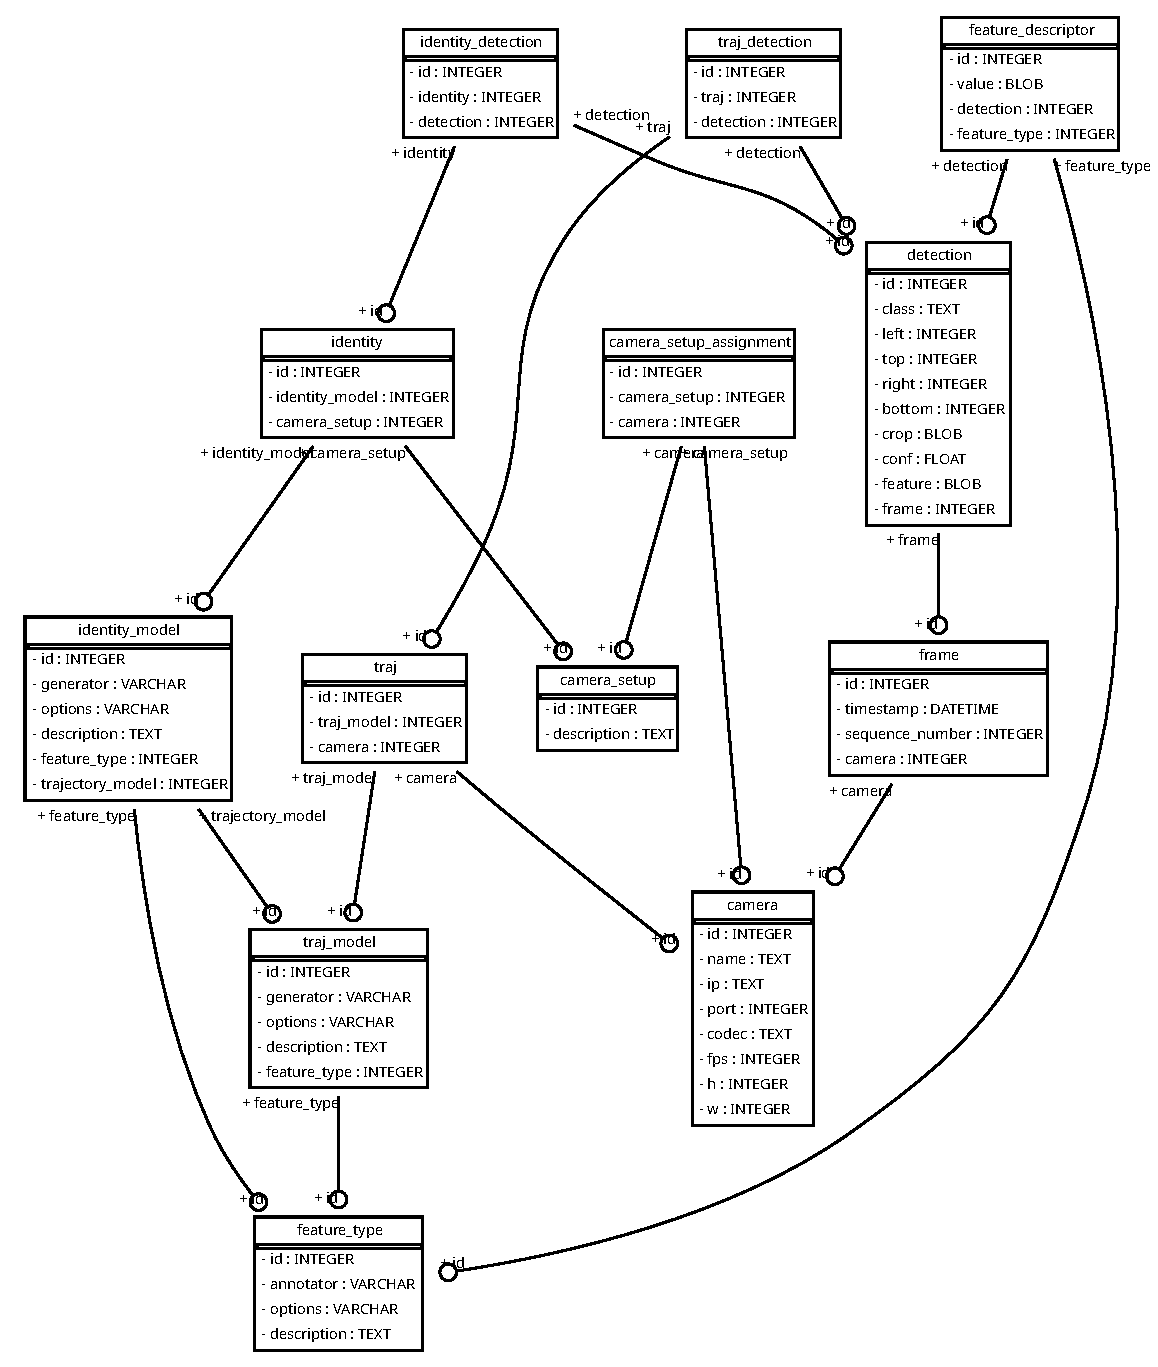
\includegraphics[width=\textwidth]{../img/database_schema.pdf}
    \caption{Schema of the Database}
    \label{fig:db_structure}
\end{figure}

\section{Input storing}

On the input our program processes \emph{detections}. Under the term \emph{detection}, we understand crops from
the frames of the camera where is an object of identification. Furthermore, we except some metadata for each
detection, such as the position within the frame and size of the crop. This information should be stored within
the \texttt{detection} table.

Alongside the information on the particular \emph{detections}, we also need a little information regarding the
original video. The information about each individual frame should are stored in the \emph{frame} table and general
information regarding the cameras (or generally, input streams) are stored in the \emph{camera} table.

Furthermore, if there are several cameras and streams that capture related scenes, such information should also be
stored in the database. In particular, for each such setup there should be a single record in the \texttt{camera\_setup}
table. Finally, there is a \texttt{camera\_setup\_assignment}. This table functions as a standard $n-\mathrm{to}-n$ connection between the \texttt{camera\_setup} table and \texttt{camera} table. This way, we encode a list of cameras for each camera setup.


\section{Feature vectors}
  
In the database, we store the per-detection feature vector as an intermediate
result. For easy testing of various feature vector types, we allow multiple
types of feature vectors to be stored per detection.

Each type of the feature vector has a record stored in the \texttt{feature\_type}
table. If the given feature vector type has various options (i.e., number of bins in
case of color histograms), there is a record for each such setting. The actual
values of given feature vectors are then stored within the \texttt{feature\_value}
table.

\section{Trajectories}

By the term \emph{trajectory} we understand a set of \emph{detections} within
single camera. In other words, they are the re-identification when we employ just
one stream.

While some re-identification algorithms generate results directly from \emph{detections},
other algorithms require existing trajectories in order to
work properly. For this reason, we also provide a few algorithms for the generation
of the \emph{trajectories}. However, this design allows for other third-party
algorithms for generating trajectories to be used. This way, we may achieve
even better re-identification results.

Similar to the feature vectors, we allow for multiple trajectories generating
models to be stored within the database. For each used algorithm, there should
be a record in \texttt{traj\_model} table, this record should include all the options
and parameters for the algorithm to ensure reproducibility.

Each trajectory (i.e., set of detections within a camera that we consider originates
from one object) has a record in \texttt{traj} table. In order to allow more comfortable and
faster querying, we also store the id of \emph{camera} by each record, this id should
match the camera id of corresponding detections.

Finally, we use the \texttt{traj\_detection} table to record of which detections
the trajectories consists of. The table functions as standard $n-\textrm{to}-n$
matching between \texttt{traj} and \texttt{detection} table.

\section{Re-identification}

Finally, we store the actual re-identification (i.e., the output of our algorithm)
in the database. The structure is generally very similar to the \emph{trajectories}. The difference is
that identities are assigned to \emph{camera setups} rather than
the \emph{cameras}. This allows for re-identification to span across several \emph{cameras}, while \emph{trajectories} are bound to a single camera.

Again, to allow evaluation of multiple approaches there is a record of each approach
in \texttt{identity\_model} table. Each actual identity is recorded in the
\texttt{identity} table. These records are also tied with \emph{camera setups}
(just as the \emph{trajectories} are tied with \emph{cameras}). Finally, the table
\texttt{identity\_detection} serves as the connection between each re-identification
and actual detections.

\chapter{Annotation tool}

Just like in any other case of a machine learning algorithm, we needed annotated data even in our case. As the videos used for development and testing the re-identification algorithm was several minutes long, there were thousands of frames and tens of thousands
of detections for annotation.

In order to make the annotation as easy as possible, we present an annotation tool that we used during the development of our algorithms. While the annotation was the primary task, we can use the tool for the exploration of results of both, various 
\emph{reidentifictaiton} algorithm and also algorithms that output just 
\emph{trajectories}.

\section{Tool options}

The annotation tool is, as other parts of this work, designed as a module of the whole
framework for in-video identification and to be used as a library. However, as the
nature of the tool requires, we also implemented a standard command-line interface.
The tool can be invoked (after installation of all dependencies) as follows:

\begin{verbatim}
$ python3 -m ReID.explore    
\end{verbatim}

A list of parameters required for the annotation tool to run can be obtained by running
the took with \texttt{\-\-help} flag. Description of various options can be seen in
figure \ref{fig:annotation_tool_help}

\begin{figure}
    \begin{verbatim}
usage: explore.py [-h] [--log {DEBUG,INFO,WARNING,ERROR,CRITICAL}]
                  -c CAMERA_IDS [CAMERA_IDS ...] [-f FILE]
                  [-t TRAJECTORY_MODEL_ID] [-i IDENTITY_MODEL_ID]
                  [-p] [--fullscreen]

optional arguments:
  -h, --help            show this help message and exit
  --log {DEBUG,INFO,WARNING,ERROR,CRITICAL}
                        Threshold for logger level
  -c CAMERA_IDS [CAMERA_IDS ...], --camera_ids CAMERA_IDS
                        [CAMERA_IDS ...] ID of camera(s) to
                        explore
  -f FILE, --file FILE  Name of the file to load trajectory model
                        from
  -t TRAJECTORY_MODEL_ID, --trajectory TRAJECTORY_MODEL_ID
                        ID of base trajectory model
  -i IDENTITY_MODEL_ID, --identity IDENTITY_MODEL_ID
                        ID of base identity model
  -p, --preload         Preload all detection in initialization
  --fullscreen, --fs    Run in fullscreen mode
  -s SCALE, --scale SCALE
                        Scale the screen of the camera(s) by given
                        factor
  -k CLASS, --class CLASS
                        If specified, show only detections of
                        given class
  --start START_TIME    Query only frames from this timestamp onwards
                        (relative to the first frame of this camera)
  --end END_TIME        Query only frames up to this timestamp (relative to
                        the first frame of this camera)


    \end{verbatim}
    \caption{Annotation tool help output}
    \label{fig:annotation_tool_help}
\end{figure}

As we already stated, the annotation tool is capable of handling both -- results of re-identification and the results of trajectory generation. From the command line we
make this distinction by either specifying the \emph{trajectory model} id (the
\texttt{\-\-trajectory} option) or the \emph{identity model} id (the
\texttt{\-\-identity} option. Either way, the selected IDs should correspond to the
ID of the model in database (form the \texttt{traj\_model} resp. 
\texttt{identity\_model}). Shown detections will then be displayed in the context
of the selected model.

Furthermore, instead of selecting direct trajectories or identifications from the
database, we can load these from the file that was generated by the previous run of
annotation tool. This may be useful if we do not want to save the annotated data
into the database but want to save the intermediate results (this way we can save
time by as these files may be stored locally, rather than uploaded on remote
server).

We select the input stream via the \texttt{\-\-camera\_ids} option. These IDs should
correspond to the IDs of cameras in the \texttt{camera} table. If we browse the
results of \emph{trajectory} detection, we may naturally select just one camera
as an input. On the other hand, if we are exploring the results of
\emph{re-identification}, we should list all the cameras that were presented
for the generation of the re-identification. The program will then find and select
appropriate \emph{camera setup} from the database.

In standard behavior, the detections are loaded on-demand. This means that the detections
are queried just after displaying their frame (unless given frame was already loaded).
As a result, the user may experience a short lag whenever he switches to a different frame.
In order to eliminate or at least minimize this delay, we implement the
\texttt{\-\-preload} option. With this flag on, all the detections are loaded on the
lunch of the tool. This will significantly prolong the start-up of the application; on the other hand, the whole experience of using the tool is smoother.

If we attempt to annotate data that comes from the source that is in higher resolution
than our current display, whole annotation tool does not fit into screen. For this case
we also implemented scaling of the display, so we can make the source detection smaller,
effectivelly fitting in our screen. Scaling option can be turned on by the
\texttt{\-\-scale} option, followed by the factor we want to scale (i.e. if we want the
source input to seem twice as small we input factor 0.5). Via the same option we can
make the detection bigger if we wish so.

If we do not want to query all the frames, we can use options \verb+--start+ and
\verb+--end+. These options will make the application to query only frames and detection
within given offset from the first frame of the stream. For example \verb+--end 00:01:00+
will cause that only frames from the first minute of the video will be loaded.
Combination of options \verb+--start 00:01:00+ and \verb+--end 00:02:00+ will load
frames from the second minute of the video. This is especially useful when used with
the \verb+--preload+ options. As normally are detections loaded on-demand there is very
little speed-up if we use \verb+--start+ and \verb+--end+ by themselves. However, when
using \verb+--preload+ all the detections are loaded at, startup; giving time interval
to load detection from can dramatically decrease number of detections loaded and thus
significantly speed-up the start up of the application.

\section{User Interface}

After launching the application, the detections from the first frame of the corresponding
camera (or cameras) are displayed. Example of such screen is shown in figure
\ref{fig:annotation_tool_screenshot}.

\begin{figure}
    \centering
    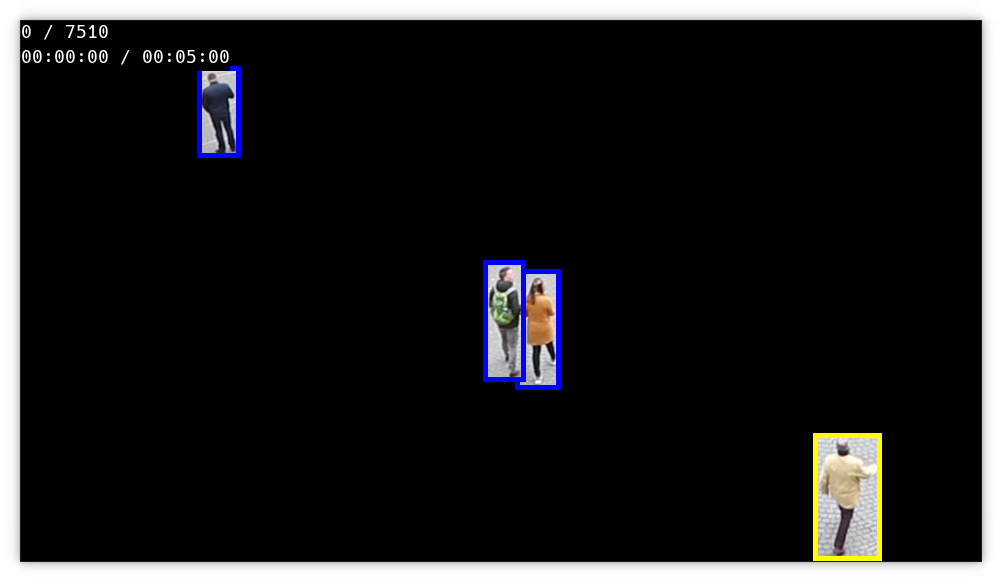
\includegraphics[width=\textwidth]{../img/annotation_tool_screenshot.png}
    \caption{Example of the first frame of the annotation tool}
    \label{fig:annotation_tool_screenshot}
\end{figure}

After launching the application, we can see highlighted detections from
the first frame of the video on the screen.
Only detections are shown, not the whole video, in this way, we do not need access
to the original video (just data already presented in the database). In the top left corner
of the screen, we can see the sequence number of the frame (this is not the frame ID
in the corresponding database, just a sequence number within the respective stream). Alongside
the sequence number is displayed the timestamp of the displayed frame.

We can browse the video by right and left arrows, skipping one frame forward and
backward, respectively. Each time we skip on a different frame, the detections from
the new frame are rendered and highlighted. However, the old detections are left
on the screen for better referencing the previous screen. The user can refresh the display
and hide all detections apart from detections from the current frame by hitting \verb+c+.
For other commands allowing to browse the stream refer to table
\ref{tab:annotation_basic_commands}

By clicking on the detection with a mouse button user can select given detection (or rather trajectory/identity of the corresponding detection). One identity can be selected
by the left mouse button and one other by the right mouse button. Selected identities can then be unified via \verb+unify+ command. One can also select a detection with the
middle mouse button. Unlike selection with the left and right mouse button, the application
allows for multiple identities to be selected with the middle mouse button. Such selection
does not serve the purpose of annotation directly (does not work with \verb+unify+ command.
However, it marks the given identity as already processed. Annotators can then use the Up and Down key for scrolling more efficiently. Refer to table 
\ref{tab:annotation_basic_commands} for further explanation of Up and Down commands.

\begin{table}
    \centering
    \begin{tabularx}{\textwidth}{l|X}
         \textbf{Key} & \textbf{Command} \\ \hline
         Right arrow & Skip one frame forward \\ \hline
         Left arrow & Skip one frame back \\ \hline
         Up arrow & Skip frames until the one with detection that is not selected
         via left, right or middle mouse button or to the end of the stream \\ \hline
         Down arrow & Skip frames backwards until the one with detection that is not selected via left, right or middle mouse button or to the first frame \\ \hline
         Page up & Skip 10 frames forward \\ \hline
         Page down & Skip 10 frames back \\ \hline
         Home & Skip to the first frame \\ \hline
         End & Skip to the last frame
    \end{tabularx}
    \caption{Basic controls of annnotation tool}
    \label{tab:annotation_basic_commands}
\end{table}

Each selection is associated with a different highlight color for given detections.
For explanation of given colors, please refer to table \ref{tab:annotation_highlight}

\begin{table}[]
    \centering
    \begin{tabularx}{\textwidth}{l|X}
         \textbf{Color} & \textbf{Explanation} \\ \hline
         Blue & Unselected detections that are assigned into an identity \\ \hline
         Yellow & Detections that are present on the frame but are not part of any
         identity for loaded model \\ \hline
         Red & Detections/identities selected via left mouse button \\ \hline
         Green & Detections/identities selected via right mouse button \\ \hline
         Cyan & Detections/identities highlighted via middle mouse buttn \\
    \end{tabularx}
    \caption{Highlight color of detections}
    \label{tab:annotation_highlight}
\end{table}

\subsection{Fast exploration of interesting detections}

\label{subsec:exploration}

Aside from the standard controlling mechanism, we offer additional features especially
useful for exploring incorrectly identified and annotated identities. We allow
for a loading list of pairs of identities during the exploration of the results. These
identities can be quickly searched through. By this method, we an, for example, efficiently fix the incorrectly annotated data in the golden dataset if we obtain a list of ``suspicious'' identities (for example list of identities that our re-identification algorithm classified differently than are classified in the golden dataset).

The list itself should state two identities ID (corresponding to the IDs in the
database) on each line, separated by space. The lines that start with the hash (\verb+#+) are considered as comments and not processed. Once the pairs are loaded
from the file with \verb+load_pairs+ command, given pairs can be processed via other
commands, refer to section \ref{sec:commands} for a complete list of commands.

\section{Commands}
\label{sec:commands}

By typing colon (\verb+:+) the user enters the command mode. Then the user can type
a command which will be displayed at the lower part of the screen. Commands are confirmed
by hitting enter and canceled via Escape. List of available command is:

\begin{itemize}
    \item \verb+unify+ (or hitting \verb+u+ in standard mode) -- merge all detections
    from identity selected by right mouse button into identity selected by left mouse 
    button
    \item \verb+hide+ (or hitting \verb+h+ in standard mode) -- hide the identity
    currently selected with the left mouse button (detections from given identity
    will be treated as if they would not be part of any identity at all, i.e.
    highlighted in yellow if all the detections are visible, or not displayed at all
    if user hid them via \verb+all+ command).
    \item \verb+all+ (or hitting \verb+a+ in standard mode) -- stops showing detections
    that are not part of any identity. If these detections are already hidden, start
    showing them instead
    \item \verb+quit+ (or hitting \verb+q+ or \verb+Esc+ in standard mode) -- terminates
    the application
    \item \verb+left+ (or hitting \verb+l+ in standard mode) -- find and skip to the
    first frame where is detection selected by left mouse button. Frames are searched
    starting from the current frame onwards (previsou frames are not searched at all)
    \item \verb+right+ (or hitting \verb+r+ in standard mode) -- works same as the 
    \verb+left+ command, except it searches for detections selected with right mouse
    button
    \item \verb+transfer+ (or hitting \verb+t+ in standard mode) -- move the detection
    from the identity selected by right mouse button that is currently displayed from
    its identity into identity selected by left mouse button.
    \item \verb+single_auto+ (or hitting \verb+s+ in standard mode) -- create new
    identity/trajectory and assign currently displayed detection that is part of the
    identity/trajectory selected by right mouse button into it.
    \item \verb+id+ (or hitting \verb+i+ in standard mode) -- start showing IDs of
    detections below the currenly highlighted detections. These correspond to the IDs
    in the \texttt{detection} table.
    \item \verb+memory+ (or hitting \verb+m+ in standard mode) -- repeat the last search 
    for deteciton (invoked with commands
    like \verb+left+, \verb+right+, \verb+find+ or \verb+next+
    \item \verb+postpone+ (or hitting \verb+p+ in standard mode) -- mark last searched 
    pair of identities as not resolved. This pair will appear in form of comment should
    the pairs be saved in this session.
    \item \verb+next+ (or hitting \verb+n+ in standard mode) -- search for next pair
    of identities loaded via \verb+load_pairs+ command. This will automatically skip
    to the first frame with the detection from the first identity. Furthermore, the
    first identity will be selected with left mouse button and the second with the
    right mouse button. Given pair will be marked as processed, meaning that it will
    not appear in the file for subsequent \verb+save_pairs+ command (unless the pair
    is postponed via \verb+postpone+ command).
    \item \verb+clear+ (or hitting \verb+c+ in standard mode) -- refresh the view.
    This will delete all the detections displayed for other frames and leaves only
    the detections from current frame.
    \item \verb+delete+ (or hitting \verb+d+ in standard mode) -- remove identity
    selected by left mouse button from the moden entirely
    \item \verb+save <file_path>+ -- store the current model into a local file
    specificied via \verb+<file_path>+ if given file does not exists
    \item \verb+save! <file_path>+ -- works same as the \verb+save+ command except
    it overrites given file if it exists
    \item \verb+upload <generator_name> <options>+ -- stores current model into the
    database as model with given parameters
    \item \verb+find <detection_id> [(l|r|<detection_id>)]+ -- skips to the frame
    with detection with given \verb+<detection_id>+. If the ID is followed by \verb+l+,
    automatically select the detection via left mouse button, if it is followed by
    \verb+r+ select it via right mouse button. If the ID is followed by second
    \verb+<detection_id>+, select the detection corresponding to the first ID by left
    mouse button, and the detection corresponding to the second ID by right mouse button
    \item \verb+single <detection_id>+ -- create a new identity/trajectory. Assign the
    detection with \verb+<detection_id>+ into it.
    \item \verb+load_pairs <file_path>+ -- load list of pairs of identities (as per subsection \ref{subsec:exploration}). 
    \item \verb+save_pairs <file_path>+ -- save all remaining pairs of identities that were loaded via \verb+load_pairs+ and not processed via \verb+next+ command. The
    pairs are saved to the corresponding \verb+<file_path>+, unless given file already
    exists
    \item \verb+save_pairs! <file_path>+ -- works the same as the \verb+save_pairs+
    command, except it overrides the file \verb+<file_path>+ if it exists
    \item \verb+select_left <identity_id>+ -- select identity \verb+<identity_id>+ 
    as with the left mouse button and
    skip to the first frame with the detection from given identity
    \item \verb+select_right <identity_id>+ -- works the same as \verb+select_left+
    command, except it select given identity with the right mouse button.
\end{itemize}

\chapter{Feature vectors}

As the first step in re-identification process, we need to extract useful information
from each detection we are tasked to identify. This process serves multiple purposes.

If we encode every useful information from the image of the detection, we can discard
the crop itself after generating the feature vector. This may significantly decrease
the amount of space we need to reserve to store the information regarding the detections.
Although, the ratio of how much memory we can save by this process heavily rely on
the fact how the feature vector is generated (and how big the final vector is).
Furthermore, if it is possible to generate the feature vectors on-line we can entirely
skip the step of storing the detections in the database and decrease the memory
requirements even further.

Other significant advantage of this process is the anonymization. Unless the generated
feature vector is reversible, we can entirely anonymize the images of potentially
sensitive images.

Nevertheless, the goal is to not supply the re-identification algorithm with the original
crop but rather corresponding feature vector. Therefor, we also need to convey
as much information in regards to identification into the feature vector as possible.
Generally, this means that we want detections to lead to the feature vectors that are
close (in terms of suitable distance, like euklidean distance) to the feature vectors
from other detections from the same identity (although details depend on the 
used re-identification algorithm).

\section{Running the Algorithm}
\label{sec:running_annotator}

All the algorithms for creating the feature vectors are implemented in the file
\texttt{ReID\/annotator.py}. The annotation process itself can be started independently
of other parts of the framework, as long as the annotated detections are already
inserted into the database.

Annotation can be started by following command:
\begin{verbatim}
    $ python -m ReID.annotator
\end{verbatim}
However, such command needs to be followed by various options and then by selected
algorithm for annotation (and then options specific for given algorithm). An example of 
complete command for annotation is:
\begin{verbatim}
    $ python -m ReID.annotator --log DEBUG -c 468 --class person\
      -p 1000 -j 8 resnet-prepare --shape 48 48
\end{verbatim}

In this case global options are (\verb+--log+, \verb+-c+ and \verb+--class+). They are 
followed by selection of specific annotating algorithm (\verb+resnet-prepare+). At 
the end of the command are options for that specific algorithm (\verb+--shape+).

\begin{figure}
    \begin{verbatim}
usage: annotator.py [--log {DEBUG,INFO,WARNING,ERROR,CRITICAL}]
                    [-h] -c CAMERA[--class CLASS] [-p PAGE_SIZE]
                    [-j JOBS] [-f] {simple-hue-histogram,
                    cropped-hue-histogram,gauss-hue-histogram,
                    resnet-prepare,mobilenet-prepare}
                    ...

positional arguments:
  {simple-hue-histogram,cropped-hue-histogram,gauss-hue-histogram,resnet-prepare,mobilenet-prepare}
                        Annotator to use for the annotation
  annotator_arguments   Additional arguments for chosen annotator

optional arguments:
  -h, --help            show this help message and exit
  --log {DEBUG,INFO,WARNING,ERROR,CRITICAL}
                        Threshold for logger level
  -c CAMERA, --camera CAMERA
                        ID of camera to annotate
  --class CLASS         Class to annotate (e.g. PERSON), if omitted all
                        classes are annotated
  -p PAGE_SIZE, --page-size PAGE_SIZE
                        Number of detection requested from database at one
                        time. Setting this to low number decreases local RAM
                        usage but increases the number of database requests.
                        To disable paging altogether, set this to 0
  -j JOBS, --jobs JOBS  Number of jobs (threads) to use
  -f, --force-update    Recompute descriptors even if they are already present
    \end{verbatim}
    \caption{Help message for annotator algorithm}
    \label{fig:annotator_help}
\end{figure}

Most of the global options are explained in the help message (obtained by using
\verb+--help+ flag) as you can see in Figure \ref{fig:annotator_help}. In standard
mode if the algorithm already finds the detections are already annotated with this
specific options if will report this error and will not run. This behavior can be
overridden by the \verb+--force-update+ option.

Other more complicated option is \verb+--page-size+. This parameter sets how many
records will be requested from the database at once. Setting this to very high number
(or disabling completely) may result in problems with unsufficient memory, as the 
algorithm needs to store at the same time that many records (most notably, images of 
detections). On the other hand, setting this to very low number will result in
significantly slower annotation as it increases number of database requests needed.
This also affect the progress bar showing number of annotated detections. The progress
bar updates after the whole batch is annotated, this means that for high number the
progress bar is updated in large intervals and for low numbers the progress bar works
far smoother.

\section{Color-based feature vectors}

As one of the more basic approachas for generation of feature vector we extract colors
from the images of detections. The idea here is that the different detection of the same
person should have roughly look same in terms of colors. Of course, if we focus on
re-identification within a single camera, spatial information will still be far more
important than such feature vector. Howerver, we can reasonably except that the colors
of the detections will remain the same even across several cameras, especially if the
cameras are will capture the object from roughly the same angle.

In order to mitigate the effect of illumination and shadows, we firstly convert the
detection images into the HSV encoding and then extract the HUE part of the encoding.
For each detection we then proceed the construct a histogram of HUE. Such histograms
should reasonably well represent the color distribution, hence the image of the same
person should be resonably similar. We will further investigate these claims in the 
Chapter \ref{ch:evaluation}.

In order to annotate the detection with such simple histograms, one can use:
\begin{verbatim}
    $ python -m ReID.annotator -c <camera_id>\
      simple-hue-histogram --bins 50
\end{verbatim}

Of course, we can use other global flags as described in Section 
\ref{sec:running_annotator}. Apart from them this annotator offers another specific
flag \verb+--bins+. This parameter describes the number of bins for the histogram.

The program will fetch all the corresponding detections, computes the histogram
of given parameters and stores them in database in form of raw numpy array
(\cite{numpy}). The images may be of varying sizes and dimensions (e.g. images
from vidoes in higer dimesnsion may have twice as many pixels as images from video
of lower resolution, making the histogram significantly different). To counter this
problem we normalize the histogram, so sizes of bins represent ratio of given color
within the image rather than absolute number of pixels with given color.

\subsection{Background elimination}

One of the problem with such basic approach is that the large part of the detection
image consists of the background. This may significantly shift general color composition
of the image and thus change the historgam.

One can notice, that the actual object is usually in the middle of the detection and the
corners are in vast majority of the cases filled with the background. Therefor, we
present few simple techniques that focuses on the middle of the image, as such focus
should capture more of the object and less of the background, making the resulting
histogram more representative.

\subsubsection{Cropped image}

The simplies possible solution for this problem is to crop the image even further 
and taking into consideration only the middle part of the image. This aproach we can
test via running the following:

\begin{verbatim}
    $ python -m ReID.annotator -c <camera_id> \
      cropped-hue-histogram\
      -b <bins> -x <from_x> <to_x> -y <from_y> <to_y>
\end{verbatim}

The \verb+--bins+ (or \verb+-b+) command works the same as in case of simple histograms.
New options \verb+-x+ and \verb+-y+ allows us to specify the crop we want to consider
for histogram generation. For each of these flags we need to specify lower and upper
boundary of $x$-axis (horizontal) and $y$-axis (vertical) axis. The boundaries are
relative to the width and height of the detection image. Thus, for example setting $x$ 
and $y$ boundaries to 0 and 1 will result in the same result as not using cropped
histogram at all. More useful example is to setting the boundaries to $0.25$ and $0.75$,
which will extract the middle part of the image. However, one may consider for $y$ axis
setting boundaries to capture part of the image closer to the top (as we usually
capture people, and this way we may evaluate torso, arguably the most telling part).
As we consider coordinate 0,0 to be top-left, to capture part of the image closer
to the top, one should set \verb+-y+ paremater for example to $0.15\,0.65$.

\subsubsection{Gaussian weighting}

We offer one more ``smoother'' approach to mitigate the influence of the background.
Rather than just consider the pixels in the middle of the image and discard the rest,
we increase the weights of the pixels closer to the middle and decrease the weight
of pixel near borders.

Most straight-forward weighting function that fulfills required properties (positivity
over whole domain, single maximum and decreasing everywhere in direction away from the
maximum) is Gaussian function. Therefore, we present another algorithm utilizing this
exact approach. Such algorithm can be run as follows:

\begin{verbatim}
    $ python -m ReID.annotator -c <camera_id> \\
      --bins <bins> -x <x> -y <y> -s <scale>
\end{verbatim}

Parameter \verb+--bins+ works same as in previous algorithms. Parameters \verb+-x+ and
\verb+-y+ sets the coordinate of the maximum weight. These are relative to the dimensions
of the crop, thus setting both to 0.5 will cause to maximum to be in the middle of the
crop, however one may wish to set the \verb+-y+ to for example 0.3 to set maximum to
upper part of the image (as discussed in previous section). Finally the \verb+-s+
parameter sets the spread of corresponding Gaussian function (again scaled to the 
relative dimensions of the image). If we set this parameter
to very small numbers, few pixels close to the coordinate with maximal importance will
essentially define the resulting histogram, while coordinates near the border will
have almost no effect. Higher the value of this parameter the weights of the pixels are
more balanced, setting this to very high number will have the same effect as not using
the weight at all (as all the pixels will have very similar weight).

The weight of a pixel at coordinates $x$ and $y$ can be described as:\footnote{note that 
in actual implementation we use probability distribution function (using scikit -- 
\cite{scipy}), so the computed values differ by a coefficient, this difference however 
does not influence the resulting histogram as we normalize it}
$$w(x,y) = \exp\left(\frac{-1}{2\sigma^2} \left[\left(\frac{x}{x_m}-x_o\right)^2 - \left(\frac{y}{y_m}-y_o\right)^2 \right]\right)$$
In this equation the $x_o$ and $y_o$ correspond to the coordinates with maximal
weight (i.e. values set by \verb+-x+ and \verb+-y+ respectivelty) and $x_m$ and $y_m$
refer to maximal boundaries (i.e. width and height of an image).
\chapter{Re-identification}
\label{ch:reidentification}


\chapter{Evaluation}
\label{ch:evaluation}

% \chapter{Title of the first chapter}

An~example citation: \cite{Andel07}

\section{Title of the first subchapter of the first chapter}

\section{Title of the second subchapter of the first chapter}


% \chapter{Title of the second chapter}

\section{Title of the first subchapter of the second chapter}

\section{Title of the second subchapter of the second chapter}


\chapter*{Conclusion}
\addcontentsline{toc}{chapter}{Conclusion}


%%% Bibliography
%%% Bibliography (literature used as a source)
%%%
%%% We employ bibTeX to construct the bibliography. It processes
%%% citations in the text (e.g., the \cite{...} macro) and looks up
%%% relevant entries in the bibliography.bib file.
%%%
%%% The \bibliographystyle command selects, which style will be used
%%% for references from the text. The argument in curly brackets is
%%% the name of the corresponding style file (*.bst). Both styles
%%% mentioned in this template are included in LaTeX distributions.

\bibliographystyle{plainnat}    %% Author (year)
% \bibliographystyle{unsrt}     %% [number]

\renewcommand{\bibname}{Bibliography}

%%% Generate the bibliography. Beware that if you cited no works,
%%% the empty list will be omitted completely.

\bibliography{bibliography}

%%% If case you prefer to write the bibliography manually (without bibTeX),
%%% you can use the following. Please follow the ISO 690 standard and
%%% citation conventions of your field of research.

% \begin{thebibliography}{99}
%
% \bibitem{lamport94}
%   {\sc Lamport,} Leslie.
%   \emph{\LaTeX: A Document Preparation System}.
%   2nd edition.
%   Massachusetts: Addison Wesley, 1994.
%   ISBN 0-201-52983-1.
%
% \end{thebibliography}


%%% Figures used in the thesis (consider if this is needed)
\listoffigures

%%% Tables used in the thesis (consider if this is needed)
%%% In mathematical theses, it could be better to move the list of tables to the beginning of the thesis.
\listoftables

%%% Abbreviations used in the thesis, if any, including their explanation
%%% In mathematical theses, it could be better to move the list of abbreviations to the beginning of the thesis.
\chapwithtoc{List of Abbreviations}

%%% Attachments to the master thesis, if any. Each attachment must be
%%% referred to at least once from the text of the thesis. Attachments
%%% are numbered.
%%%
%%% The printed version should preferably contain attachments, which can be
%%% read (additional tables and charts, supplementary text, examples of
%%% program output, etc.). The electronic version is more suited for attachments
%%% which will likely be used in an electronic form rather than read (program
%%% source code, data files, interactive charts, etc.). Electronic attachments
%%% should be uploaded to SIS and optionally also included in the thesis on a~CD/DVD.
%%% Allowed file formats are specified in provision of the rector no. 72/2017.
\appendix
\chapter{Attachments}

\section{First Attachment}

\openright
\end{document}
